% The document class supplies options to control rendering of some standard
% features in the result.  The goal is for uniform style, so some attention 
% to detail is *vital* with all fields.  Each field (i.e., text inside the
% curly braces below, so the MEng text inside {MEng} for instance) should 
% take into account the following:
%
% - author name       should be formatted as "FirstName LastName"
%   (not "Initial LastName" for example),
% - supervisor name   should be formatted as "Title FirstName LastName"
%   (where Title is "Dr." or "Prof." for example),
% - degree programme  should be "BSc", "MEng", "MSci", "MSc" or "PhD",
% - dissertation title should be correctly capitalised (plus you can have
%   an optional sub-title if appropriate, or leave this field blank),
% - dissertation type should be formatted as one of the following:
%   * for the MEng degree programme either "enterprise" or "research" to
%     reflect the stream,
%   * for the MSc  degree programme "$X/Y/Z$" for a project deemed to be
%     X%, Y% and Z% of type I, II and III.
% - year              should be formatted as a 4-digit year of submission
%   (so 2014 rather than the academic year, say 2013/14 say).

\documentclass[author={Jacob Stephenson},
    degree={BSc},
    title={Robust Localisation and Recognition of Great Apes in Wild Camera Trap Imagery},
    unit={COMS30045},
    subtitle={}]{dissertation}

\usepackage{amsmath,amssymb}
\usepackage{booktabs}
\usepackage{graphicx}
\usepackage{multirow}
\usepackage{subcaption}
\usepackage{tikz}

\usetikzlibrary{shapes.geometric, arrows.meta, positioning}

\tikzstyle{startstop} = [rectangle, rounded corners, minimum width=3cm, minimum height=1cm,text centered, draw=black]
\tikzstyle{process} = [rectangle, minimum width=3.5cm, minimum height=1.2cm, text centered, draw=black]
\tikzstyle{arrow} = [thick,->,>=stealth]
\tikzstyle{process} = [
    rectangle,
    text width=4cm,
    align=center,
    minimum height=1.2cm,
    draw=black
]

\date{5th May 2026}

\begin{document}

% =============================================================================

% This macro creates the standard UoB title page by using information drawn
% from the document class (meaning it is vital you select the correct degree 
% title and so on).

\maketitle

% After the title page (which is a special case in that it is not numbered)
% comes the front matter or preliminaries; this macro signals the start of
% such content, meaning the pages are numbered with Roman numerals.

\frontmatter


%\lstlistoflistings

% The following sections are part of the front matter, but are not generated
% automatically by LaTeX; the use of \chapter* means they are not numbered.

% -----------------------------------------------------------------------------

\chapter*{Abstract}



% -----------------------------------------------------------------------------


\chapter*{Dedication and Acknowledgements}

\begin{itemize}
    \item I acknowledge the use of resources provided by the Isambard-AI National AI Research Resource (AIRR). Isambard-AI is operated by the University of Bristol and is funded by the UK Government’s Department for Science, Innovation and Technology (DSIT) via UK Research and Innovation; and the Science and Technology Facilities Council [ST/AIRR/I-A-I/1023]. \cite{mcintoshsmith2024isambardaileadershipclasssupercomputer}
\end{itemize}



% -----------------------------------------------------------------------------

% This macro creates the standard UoB declaration; on the printed hard-copy,
% this must be physically signed by the author in the space indicated.

\makedecl


% -----------------------------------------------------------------------------

% This macro creates the AI declaration; on the printed hard-copy,
% this must be physically signed by the author in the space indicated.

\makeaidecl



% -----------------------------------------------------------------------------

% LaTeX automatically generates a table of contents, plus associated lists 
% of figures and tables.  These are all compulsory parts of the dissertation.

\tableofcontents
\listoffigures
\listoftables

% -----------------------------------------------------------------------------



\chapter*{Ethics Statement}




% -----------------------------------------------------------------------------

\chapter*{Summary of Changes}



% -----------------------------------------------------------------------------

\chapter*{Supporting Technologies}

\begin{itemize}
    \item I used Segment Anything Model 3 (SAM 3) \cite{carion2025sam3segmentconcepts} to evaluate the performance of existing localisation technology.
    \item I used OpenCV \cite{opencv_library} for basic operations (e.g., get video width/height), and to draw bounding boxes over copies of videos for visualisation and qualitative analysis.
    \item I used Isambard-AI Phase 2 \cite{mcintoshsmith2024isambardaileadershipclasssupercomputer} for computationally expensive operations such as segmenting large batches of videos.
\end{itemize}



% -----------------------------------------------------------------------------

\chapter*{Notation and Acronyms}

% \begin{quote}
% \noindent
% \begin{tabular}{lcl}
% AES                 &:     & Advanced Encryption Standard                                         \\
% DES                 &:     & Data Encryption Standard                                             \\
%                     &\vdots&                                                                      \\
% ${\mathcal H}( x )$ &:     & the Hamming weight of $x$                                            \\
% ${\mathbb  F}_q$    &:     & a finite field with $q$ elements                                     \\
% $x_i$               &:     & the $i$-th bit of some binary sequence $x$, st. $x_i \in \{ 0, 1 \}$ \\
% \end{tabular}
% \end{quote}

\begin{quote}
\noindent
\begin{tabular}{lcl}
    (m)AP & : & (mean) Average Precision \\
    CNN & : & Convolutional Neural Network \\
    GT & : & Ground Truth \\
    IDF1 & : & Identification F1-score \\
    MAT & : & Multi-Animal Tracking \\
    MOTA & : & Multiple Object Tracking Accuracy \\
    PCS & : & Promptable Concept Segmentation \\
    SA-FARI & : & Segment Anything in Footage of Animals for Recognition and Identification \\
    SAM 3 & : & Segment Anything Model 3 \\
\end{tabular}
\end{quote}



% =============================================================================

% After the front matter comes a number of chapters; under each chapter,
% sections, subsections and even subsubsections are permissible.  The
% pages in this part are numbered with Arabic numerals.  Note that:
%
% - A reference point can be marked using \label{XXX}, and then later
%   referred to via \ref{XXX}; for example Chapter\ref{chap:context}.
% - The chapters are presented here in one file; this can become hard
%   to manage.  An alternative is to save the content in seprate files
%   the use \input{XXX} to import it, which acts like the #include
%   directive in C.

\mainmatter


\chapter{Introduction}
\label{chap:intro}

% Potential figures:
% Camera trap screenshots
% SAM 3 model
% Project pipeline overview figure <- suggested by Tilo

\section{Context}

\subsection{Camera Trap Imagery and The Collection-Analysis Gap}

Camera trap imagery is a wildly used method for observing wildlife populations in their natural habitat. These cameras can be deployed and left to record thousands of videos, reducing the need for conventional direct human observation methods to collect data on animal presence and behaviours~\cite{Tuia_2022}. The Pan~African program are using this technique across 18 field sites in Africa to capture videos of great apes, particularly chimpanzees and gorillas~\cite{brookes2024panaf20k}.

\begin{figure}[h]
    \centering
    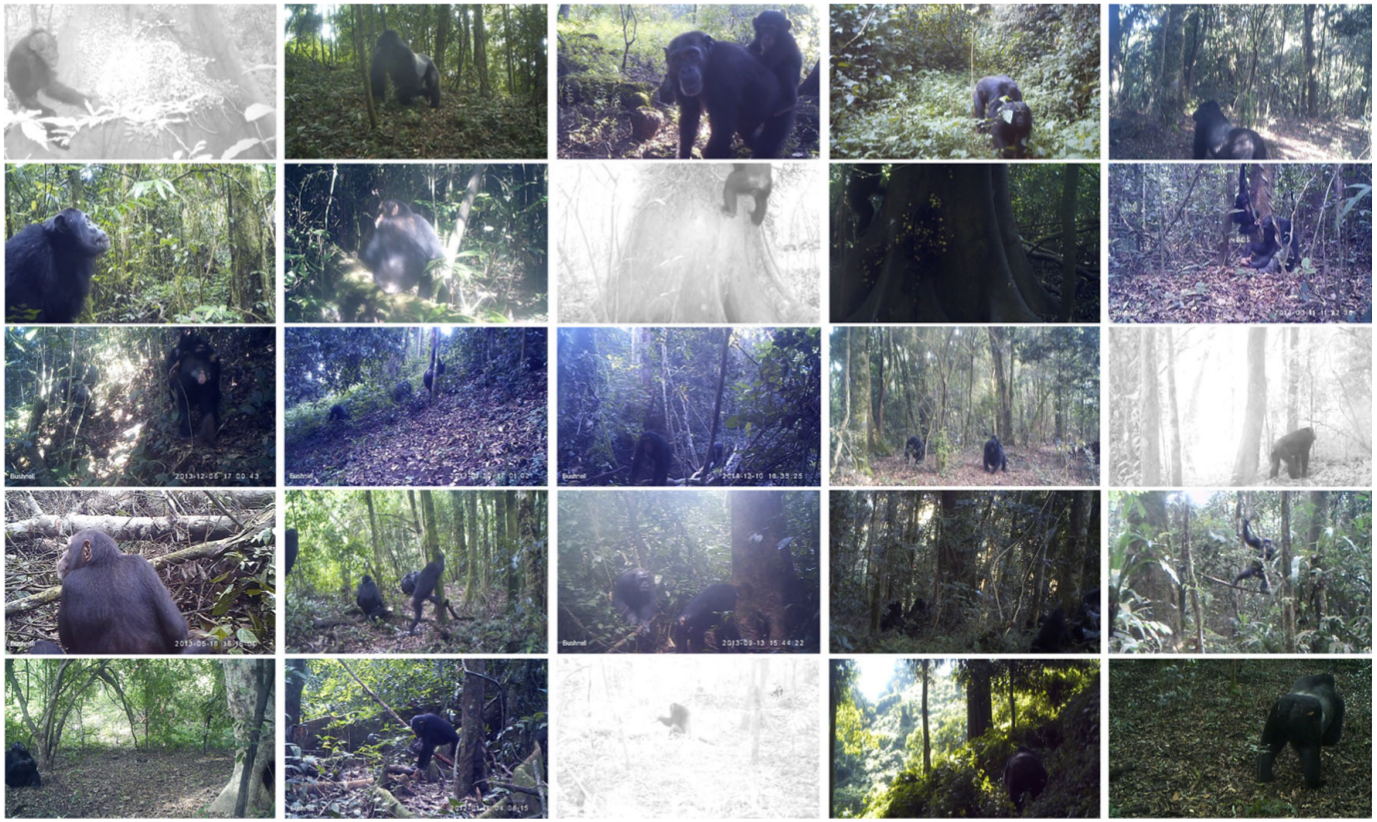
\includegraphics[width=\textwidth]{images/panaf.png}
    \caption[PanAf20K Camera Trap Imagery]{Example screenshots from the PanAf20K dataset. \textit{Reproduced from~\cite{brookes2024panaf20k}}.}
    \label{fig:panaf}
\end{figure}

The large amount of data generated by such projects unfortunately far exceeds what could be manually reviewed by humans; one camera alone can generate thousands of videos, some of which contain no animals at all~\cite{beery2019efficientpipelinecameratrap}. Evidently, there is a gap between data collection and analysis, which must be bridged by automated analysis methods.


\subsection{The Automation Bridge}

MegaDetector is a tool designed to filter out empty frames and localise objects (animals, people etc.) in videos~\cite{beery2019efficientpipelinecameratrap}, helping to alleviate the above problem. This works as an effective start to improving automated detection, but the main limitation is that it is not designed to identify the exact species of an animal. Therefore, in scenarios where there are multiple animals sharing a habitat, we still require human, manual classification of the localised objects.

Recent computer vision models open up the potential to solve this problem. Segment Anything Model~3 (SAM~3),designed by Meta~AI, enables spatio-temporal segmentation of images and videos, prompted with a short text phrase, referred to as Promptable Concept Segmentation (PCS)~\cite{carion2025sam3segmentconcepts}. This capability is directly relevant to camera trap analysis, but being a general purpose model, further refinement could be required before such a model could be relied on in this domain.

\begin{figure}[h]
    \centering
    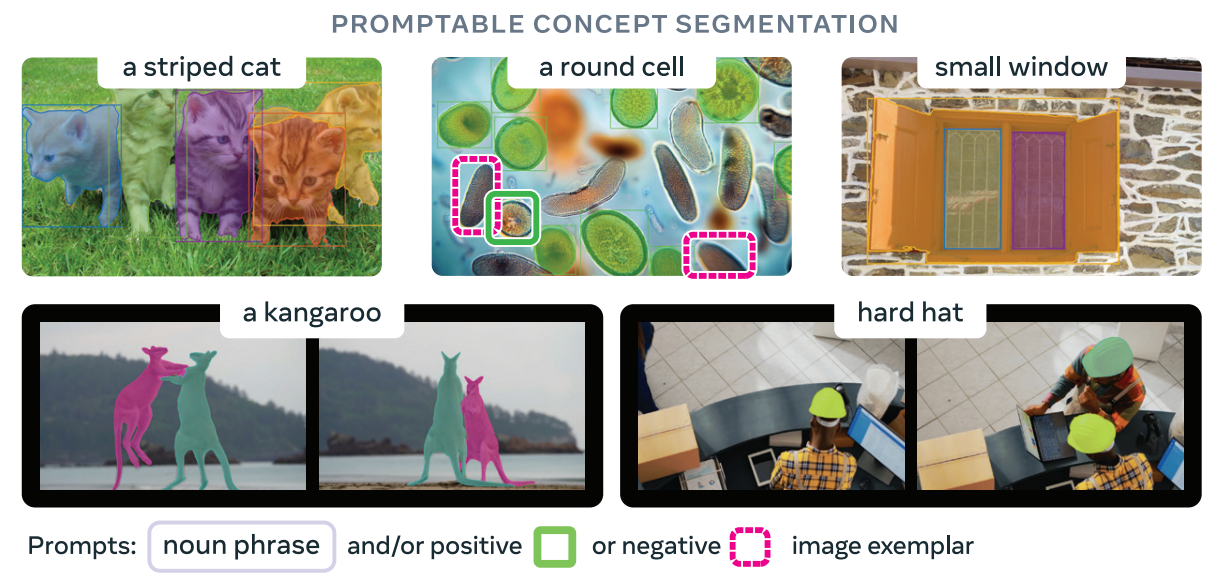
\includegraphics[width=0.8\textwidth]{images/sam3.png}
    \caption[SAM 3 Usage Examples]{Examples highlighting SAM~3's usage of PCS, allowing users to segment all instances of an object specified by a short text prompt. \textit{Reproduced from \cite{carion2025sam3segmentconcepts}}}
    \label{fig:sam3}
\end{figure}

Alongside SAM~3, the SA-FARI dataset was released, as well as the fine-tuned model weights derived from the dataset, aiming to improve on the default model for this purpose~\cite{wasmuht2025safaridatasetsegmentfootage}. This dataset contains a wide variety of animals between 741 field sites, including chimpanzees and gorillas from the PanAf program, videos which will be used to conduct the research in this work.

Despite the advantages, the task of robust and reliable localisation of great apes in wild camera trap footage presents several challenges. For one, the apes can appear in conventionally difficult computer vision environments, such as low quality video, variable lighting, occluded environments, at a distance from the camera or facing away from the lens \cite{brookes2024panaf20k, yang2019greatapedetectionchallenging}. Furthermore, chimpanzees and gorillas share many visually similar features, being large-bodied species with dark fur. In some of the challenging environments mentioned, it can be difficult for even a human to differentiate between the two species. It is also unclear what knowledge SAM~3 leverages to identify apes: does it have a general idea of what an ape looks like, or can it use species specific information to come to an informed decision?


\section{Aims and Objectives}

This work takes an exploratory approach to investigating these problems and questions. Rather than working around a fixed hypothesis, we work through a series of investigations, with each one motivated by the last. First, we evaluate SAM~3's baseline performance with a variety of configurations, including basic prompts and alternate model weights. Then, we investigate whether a prompt engineering approach can be used to yield more desired outputs, as this is an under explored approach. Finally, after establishing the limits posed by this approach, we design two purpose built classification models, a custom CNN and a fine-tuned ResNet-18~\cite{he2015deepresiduallearningimage} model, proposing the practicality of using such a model in combination with SAM~3 to alleviate some of the shortfalls of using the model alone.

The project aims to improve the robustness of localisation of great apes in wild camera trap imagery, but more concretely, the aims and objectives are as follows:

\begin{enumerate}
    \item Develop an initial understanding of SAM~3's performance, including common success and failure cases, in localising, tracking and classifying great apes.
    \item Investigate the impact of prompt engineering in improving SAM~3 detection accuracy and species-level discrimination.
    \item Design and compare two-way species classifiers, leveraging SAM~3 outputs as training data.
    \item Propose a segmentation-classification pipeline, integrating SAM~3 with the best-performing classifier to improve species-level discrimination.
\end{enumerate}

\medskip

\begin{figure}[h]
\centering
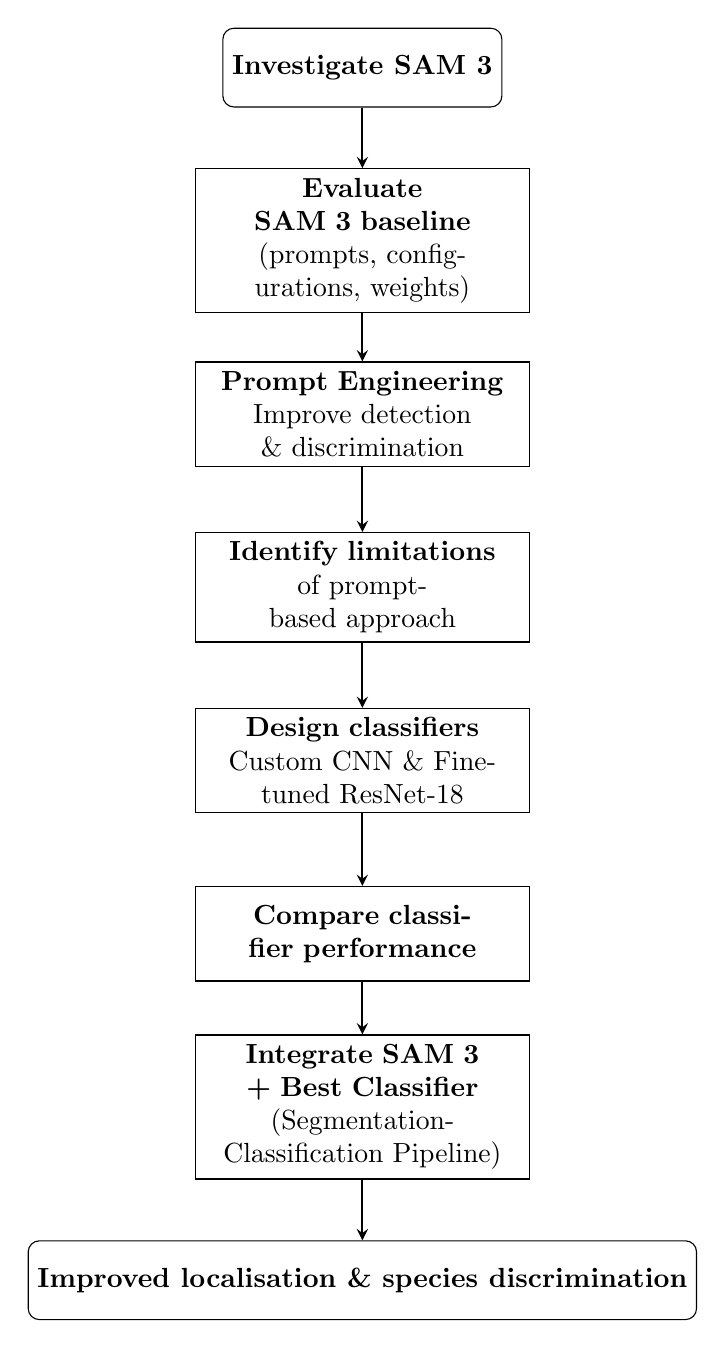
\begin{tikzpicture}[node distance=2.2cm]

% Nodes
\node (start) [startstop] {\textbf{Investigate SAM~3}};

\node (eval) [process, below of=start] 
{\textbf{Evaluate SAM~3 baseline}\\
(prompts, configurations, weights)};

\node (prompt) [process, below of=eval] 
{\textbf{Prompt Engineering}\\
Improve detection \& discrimination};

\node (limit) [process, below of=prompt] 
{\textbf{Identify limitations}\\
of prompt-based approach};

\node (models) [process, below of=limit] 
{\textbf{Design classifiers}\\
Custom CNN \& Fine-tuned ResNet-18};

\node (compare) [process, below of=models] 
{\textbf{Compare classifier performance}};

\node (pipeline) [process, below of=compare] 
{\textbf{Integrate SAM~3 + Best Classifier}\\
(Segmentation-Classification Pipeline)};

\node (end) [startstop, below of=pipeline] 
{\textbf{Improved localisation \& species discrimination}};

% Arrows
\draw [arrow] (start) -- (eval);
\draw [arrow] (eval) -- (prompt);
\draw [arrow] (prompt) -- (limit);
\draw [arrow] (limit) -- (models);
\draw [arrow] (models) -- (compare);
\draw [arrow] (compare) -- (pipeline);
\draw [arrow] (pipeline) -- (end);

\end{tikzpicture}
\caption[Project Pipeline]{Project Pipeline}
\label{fig:pipeline}
\end{figure}



% -----------------------------------------------------------------------------

\chapter{Background}
\label{chap:bg}

\section{Camera Trap Monitoring of Great Apes}

\subsection{PanAf20K}

PanAf20K is a set of 20,000 static camera trap videos (roughly 7 million frames) featuring chimpanzees and gorillas in their natural habitats, \cite{brookes2024panaf20k, brookes2024panaf20kdataset} taken across 18 field sites in tropical Africa.

PanAf20K contains a fully annotated subset of 500 videos (over 180K frames), referred to as PanAf500. These fine-grained annotations feature species classification, behavioural actions, bounding boxes and associated intra-video tracking IDs. The remainder of PanAf20K contain multi-label annotations indicating behaviours present in the video without associated apes or spacial locations.

Because a subset of PanAf500 was used to train the SA-FARI model weights, the remaining 71 videos, which we shall refer to as PanAf71, were used for the initial evaluation of SAM~3 performance in Chapter~\ref{chap:execution}.

\begin{figure}[h]
    \centering
    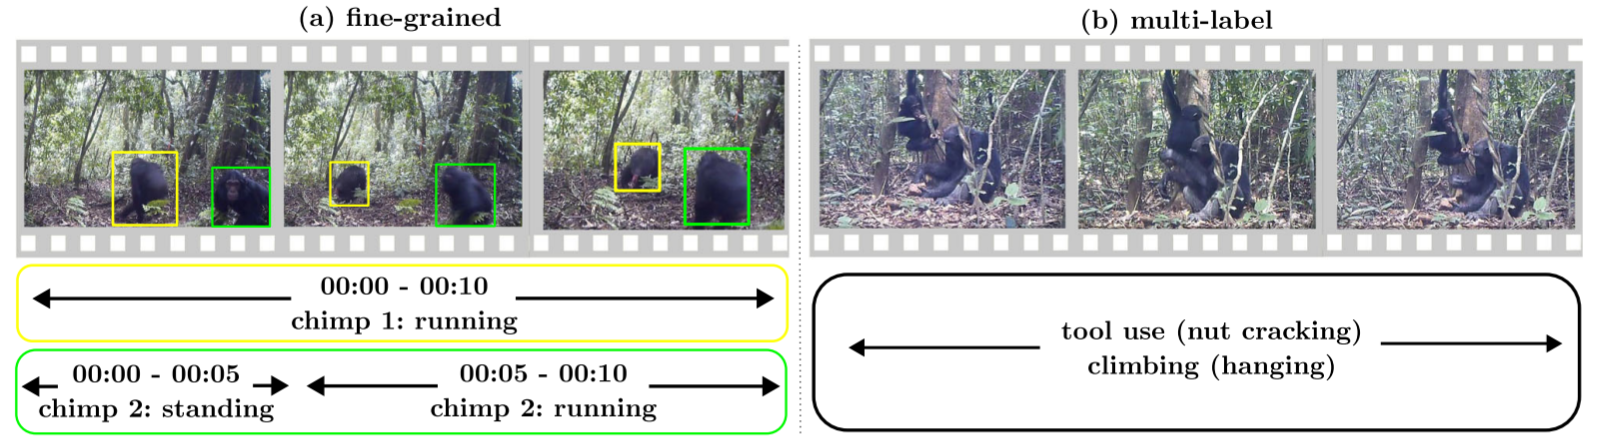
\includegraphics[width=\textwidth]{images/ape_annotations.png}
    \caption[PanAf20K Annotations]{Examples of annotations for PanAf20K. PanAf500 annotations (left) feature tight full-body bounding boxes, and frame-level behavioural actions assigned to each ape. PanAf20K annotations (right) provide only video-level behavioural annotations, without bounding boxes or ape assignment. \textit{Reproduced from \cite{brookes2024panaf20k}}}
    \label{fig:annotations}
\end{figure}

\subsection{Challenges}

The task of recognising great apes in the wild, despite being simple for humans, comes with a distinct set of challenges.

% Need citation here about camera trap imagery
First, all imagery used in this project (and the majority of data available) comes from camera traps, being static, motion-triggered cameras which are deployed in the wild for extended periods of time. The imagery generated by these cameras can be identified by their distinctly low quality and significant lighting variation between day and night shots, which, despite being a cost-effective method for monitoring animals in the wild, makes effective localisation difficult. Additionally, their static nature often leads to partial or full occlusion when animals move behind vegetation in the frame.

The occlusion is not the only roadblock posed by the forest environments; dark features such as tree branches can often be misclassified as an ape's arm for example, particularly when lighting quality is poor and the objects are far from the camera.

Finally, the videos used in this project feature chimpanzees and gorillas, who share strong visual similarity. This problem is amplified when objects are occluded, not facing the camera, or far away from it, making species-level classification non-trivial even for humans.


\section{Object Detection and Segmentation in Wildlife Imagery}




\section{Segment Anything Model 3 (SAM 3)}

SAM 3 is a foundation model for Promptable Concept Segmentation (PCS) released by Meta \cite{carion2025sam3segmentconcepts}. Given a text prompt (e.g. ``chimpanzee"), SAM 3 identifies all corresponding instances in images and videos by producing bounding boxes and segmentation mask sequences (``masklets") in the spatio-temporal domain.

In this project, SAM 3 was employed to obtain segmentation information from a varied set of videos containing chimpanzees and gorillas.


\section{Datasets}

\subsection{The SA-FARI Dataset}

SA-FARI is the largest open-source Multi-Animal Tracking (MAT) dataset for wild animals \cite{wasmuht2025safaridatasetsegmentfootage}. It contains over 11,000 camera trap videos, each with manually verified, spatio-temporal segmentation annotations.

In the context of this project, the fine-tuned model weights derived from the dataset were loaded into SAM 3 as an alternate configuration to compare species-specific performance against the out-of-the-box model weights.



\section{Evaluation Metrics}

To characterise spatial accuracy, the F1-score and AP (Average Precision) \cite{cvalgosmetrics} were adopted. To quantify tracking performance, MOTA (Multiple Object Tracking Accuracy) and IDF1 (Identification F1-score) \cite{MOTmetrics} were adopted.


\section{Taxonomy}

Taxonomy is a branch of biology concerned with classifying organisms into groups, ensuring a standardised way to refer to species \cite{britannica_taxonomy, nhm_taxonomy}.

Practically, these groups are arranged in a hierarchical ranking system. These ranks, from broadest to most specific are Domain, Kingdom, Phylum, Class, Order, Family, Genus and Species. Each step down the hierarchy represents a more specific grouping, such that species in the same genus are more closely related than those only sharing the same family.

In this project, taxonomy is used a framework for prompt design. Using the different levels of abstraction, it is possible to investigate how such prompts impact model behaviour. It is hypothesised that broader terms will increase recall, while more specific terms will improve precision.



% -----------------------------------------------------------------------------

\chapter{Project Execution}
\label{chap:execution}

\section{Initial SAM 3 Performance Evaluation}
\label{sec:execution_initial}

To identify SAM~3's strengths and weaknesses, we must first develop an initial understanding of the model's success and failure points.

\subsection{Method}

The investigation setup is as follows:
\begin{enumerate}
    \item Prepare each video from PanAf71 for processing.
    \item Provide SAM~3 with a prompt (e.g. ``ape").
    \item Load the model with either the default weights, or the fine-tuned SA-FARI weights
    \item Process each video, obtaining segmentation outputs.
    \item Evaluate model performance by comparing outputs with ground truth data, with an IoU threshold of 0.5. Note that if the prompt was species-specific (e.g. ``chimpanzee") the ground truth set was reduced to contain only the bounding boxes associated with chimpanzees.
\end{enumerate}

\begin{figure}[h]
    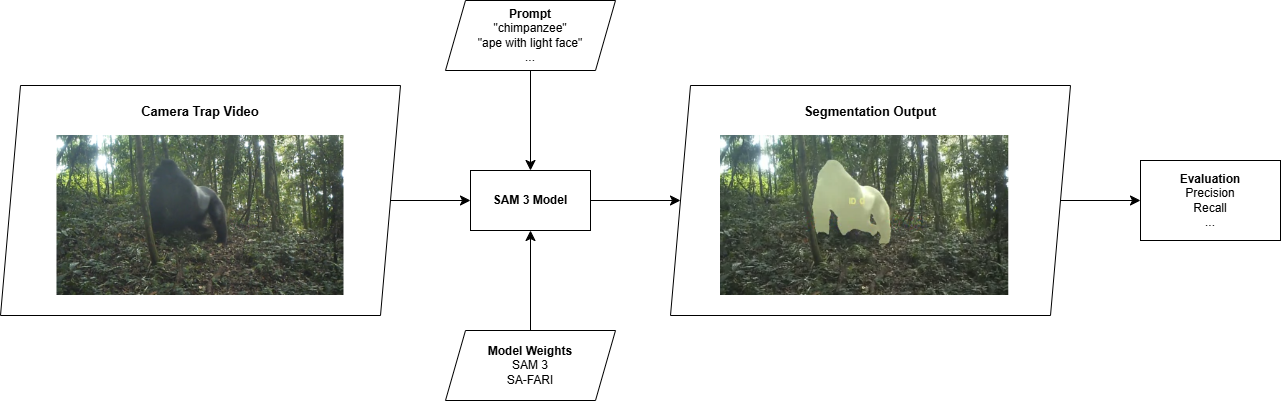
\includegraphics[width=\textwidth]{images/Flowchart.png}
    \caption[SAM~3 Evaluation Process]{Flowchart describing the SAM~3 evaluation process}
\end{figure}


\subsection{Results and Discussion}

\begin{table}[h]
    \centering
    \small
    \setlength{\tabcolsep}{4pt}

    \begin{tabular}{lll|cccc|cc}
        \toprule
        
        \textbf{Prompt} & \textbf{Target Class} & \textbf{Weights} & \textbf{Precision} & \textbf{Recall} & \textbf{F1} & \textbf{mAP} & \textbf{MOTA} & \textbf{IDF1} \\

        \midrule
        
        \multirow{2}{*}{``ape"}
            & \multirow{2}{*}{All}
            & SAM 3 & 0.42 & \underline{0.94} & 0.58 & 0.74 & -0.39 & 0.16 \\
            & & SA-FARI & \textbf{0.60} & 0.92 & \textbf{0.73} & \textbf{0.77} & \textbf{0.31} & \textbf{0.31} \\

        \midrule

        \multirow{2}{*}{``chimpanzee and gorilla"}
            & \multirow{2}{*}{All}
            & SAM 3 & 0.50 & 0.90 & 0.64 & 0.68 & -0.03 & 0.22 \\
            & & SA-FARI & 0.57 & 0.89 & 0.69 & 0.70 & 0.20 & 0.25 \\

        \midrule

        \multirow{2}{*}{``gorilla and chimpanzee"}
            & \multirow{2}{*}{All}
            & SAM 3 & 0.53 & 0.91 & 0.67 & 0.70 & 0.10 & 0.25 \\
            & & SA-FARI & 0.58 & 0.93 & 0.71 & \textbf{0.77} & 0.24 & 0.28 \\

        \midrule
        
        \multirow{2}{*}{``chimpanzee"}
            & \multirow{2}{*}{Chimpanzees}
            & SAM 3 & 0.29 & 0.94 & 0.44 & 0.64 & -1.42 & 0.15 \\
            & & SA-FARI & 0.38 & 0.94 & 0.54 & 0.62 & -0.63 & 0.30 \\

        \midrule

        \multirow{2}{*}{``gorilla"}
            & \multirow{2}{*}{Gorillas}
            & SAM 3 & 0.17 & \textbf{0.95} & 0.28 & 0.30 & -3.81 & 0.08 \\
            & & SA-FARI & 0.18 & 0.91 & 0.30 & 0.28 & -3.18 & 0.09 \\

        \bottomrule
    \end{tabular}

    \caption[Initial SAM 3 Performance Evaluation]{Metrics quantifying SAM 3 performance on the same batch of videos for different text prompts and model checkpoints. `SAM 3' denotes the default pretrained weights. `SA-FARI' refers to weights fine-tuned using positive samples only. The \textbf{Target Class} column describes the subset of annotations against which predictions were evaluated: either the whole set (All), or exclusively the annotations containing a single species. Bold values are the highest in their column. Underline shows the configuration resulting in the highest recall, specifically for species non-specific segmentation.}
    \label{tab:metricsinitial}
\end{table}

\begin{figure}[h]
    \centering
    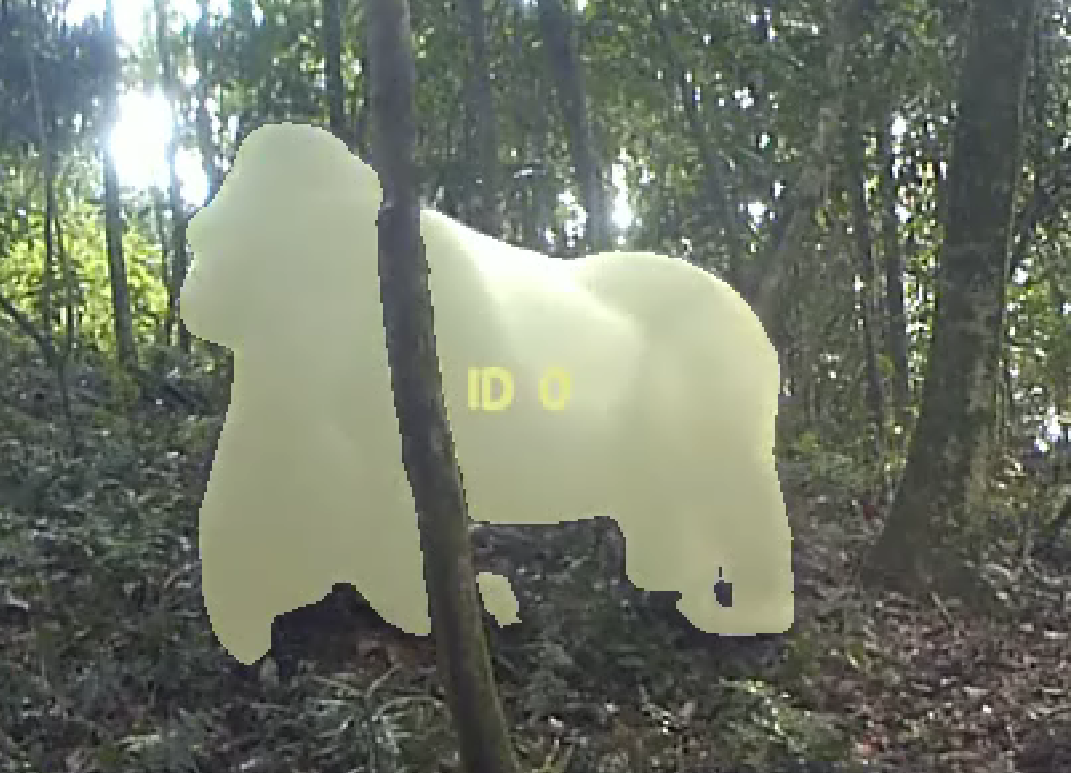
\includegraphics[width=0.37\textwidth]{images/ape_misclassification.png}
    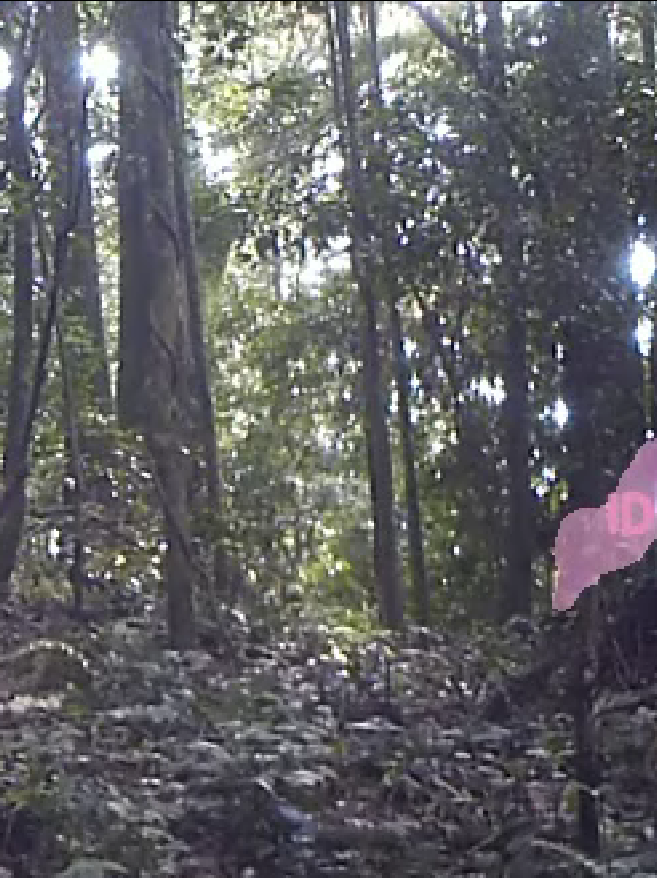
\includegraphics[width=0.2\textwidth]{images/background_fp.png}
    \caption[SAM 3 Failure Cases]{Two screenshots taken from different frames of the same video, with masks generated by prompt ``chimpanzee" and SA-FARI weights show common failure cases. The incorrect species being detected, in this case a gorilla (left), and a dark area of foliage being raised as a candidate (right).}
    \label{fig:sam3failures}
\end{figure}

The results in Table~\ref{tab:metricsinitial} demonstrate several trends. First, the SAM~3 weights typically outperform SA-FARI in recall, whereas SA-FARI consistently outperforms SAM~3 in precision. Second, the precision of species-specific predictions shown in the bottom two rows is substantially lower than the precision of species non-specific predictions. Metrics computed with tracking information (MOTA, IDF1) show consistently low tracking performance, with MOTA often being negative. Finally, despite ``chimpanzee and gorilla" and ``gorilla and chimpanzee" being semantically equivalent statements, the prompts yield differing results.

The poor tracking performance is likely a result of a combination of high false positive rates and identity switches between frames. The negative MOTA scores indicate that there are more identity switches, false negatives and false positives than ground truth objects, with high false positive rates in species-specific prompts explaining the dramatically negative MOTA scores, and IDF1 scores close to 0.

The difference in precision and recall between the two sets of weights likely reflects the behaviour of each model. SAM~3's higher recall indicates that more predictions are made, resulting in fewer missed detections and a greater number of incorrect detections. To contrast, SA-FARI produces significantly higher precision, suggesting that predictions are made more conservatively, reducing incorrect detections at the cost of increasing missed detections. Additionally, SA-FARI's higher precision was expected, as this model was specifically designed to segment animals, including chimpanzees and gorillas \cite{wasmuht2025safaridatasetsegmentfootage}.


The difficulty in distinguishing between the two ape species across both models is also evident from the results. The species specific predictions maintain high recall, but the drastic decrease in precision indicates that many of the detections correspond to the incorrect species, further supported by Figure~\ref{fig:sam3failures}. This suggests that the models rely more heavily the broader ape features than on species specific traits. Given the visual similarity of the two species in many frames, particularly those in which the object is far from the camera, partially occluded or is facing away, the models seem to detect apes fairly reliably, but struggle to differentiate between the two. Evidently, in a scenario where species-level accuracy is essential, there is significant limitation that must be refined.

Demonstrated by the semantically equivalent prompts containing ``and", SAM~3 is sensitive to prompt formulation. Thus, an investigation into prompt design was undertaken to determine whether it could improve detection performance.


\section{Prompt Investigation}
\label{sec:execution_prompt}

In this section, a 20-video subset of those used in Section~\ref{sec:execution_initial}, containing 10 videos that feature only gorillas, and 10 videos that feature only chimpanzees, was adopted. For each prompt, the model was loaded with the SA-FARI weights, and predictions were made on all 20 videos. These outputs were then evaluated against the appropriate target classes.

\subsection{Formulations}
\label{subsec:prompt_formulations}

A variety of prompt formulations were investigated, after the results in Table~\ref{tab:metricsinitial} demonstrated that the way prompts are worded affects output, evidenced by the varied results between semantically equivalent statements. These formulations include:

\begin{itemize}
    \item Single words (e.g. ``chimpanzee")
    \item Inclusion of indefinite articles (e.g. ``a chimpanzee")
    \item Negatives (e.g. ``chimpanzee and not gorilla")
\end{itemize}

\begin{table}[h]
    \centering

    \begin{tabular}{ll|cccc}
            \toprule
    
            \textbf{Prompt} & \textbf{Target Class} & \textbf{Precision} & \textbf{Recall} & \textbf{F1} & \textbf{mAP} \\

            \midrule
            
            ``ape" & All & \textbf{0.64} & 0.87 & \textbf{0.74} & \textbf{0.70} \\
            
            ``chimpanzee" & Chimpanzees & 0.28 & \textbf{0.93} & 0.43 & 0.38 \\
            
            ``gorilla" & Gorillas & 0.29 & 0.86 & 0.43 & 0.42 \\

            \midrule

            ``an ape" & All & 0.63 & 0.87 & 0.73 & \textbf{0.70} \\
            
            ``a chimpanzee" & Chimpanzees & 0.28 & 0.92 & 0.43 & 0.38 \\
            
            ``a gorilla" & Gorillas & 0.29 & 0.87 & 0.43 & 0.44 \\
    
            \midrule
            
            ``chimpanzee and not gorilla" & Chimpanzees & 0.28 & \textbf{0.93} & 0.43 & 0.37 \\
            
            ``chimpanzee rather than gorilla" & Chimpanzees & 0.27 & 0.92 & 0.42 & 0.36 \\

            ``gorilla and not chimpanzee" & Gorillas & 0.29 & 0.86 & 0.43 & 0.44 \\
    
            ``gorilla rather than chimpanzee" & Gorillas & 0.28 & 0.86 & 0.42 & 0.44 \\
            
            \bottomrule
    \end{tabular}

    \caption[Prompt formulations]{Performance of multiple prompt formulations evaluated on the 20-video subset. Note that the performance of prompts ``ape", ``chimpanzee" and ``gorilla" differs from Table~\ref{tab:metricsinitial} because of the video set used.}
    \label{tab:promptformulations}
\end{table}

\begin{figure}[h]
    \centering
    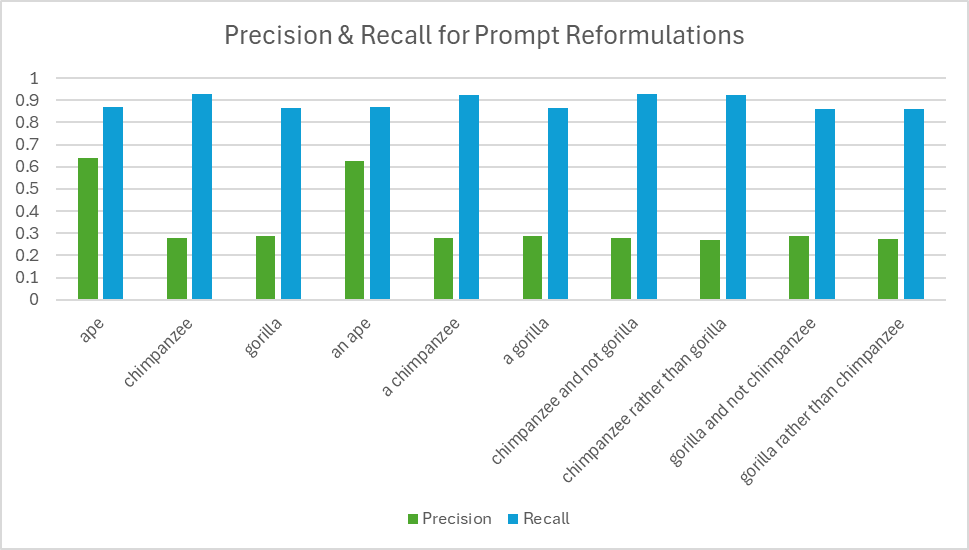
\includegraphics[width=0.75\textwidth]{images/formulations.png}
    \caption[Precision and Recall for Prompt Reformulations]{Bar chart visualising the difference in precision and recall for prompt reformulations.}
    \label{fig:promptformulations}
\end{figure}

First, a similar performance for single words can be seen in this subset compared to the set used in Section~\ref{sec:execution_initial}. Second, though including indefinite articles in prompts causes differing output, the change in performance compared to excluding them is negligible. Finally, though it was hypothesised that negatives would improve species-level precision, the majority of cases showed slightly worse precision.

These findings suggest that SAM~3 is insensitive to subtle variations in prompts. While outputs are somewhat altered by wording, it proves an ineffective method for improving performance. Thus, a more structured approach based on biological taxonomy was explored.

\subsection{Taxonomy}
\label{subsec:prompt_taxonomy}

Prompts were designed around all ranks of the taxonomy hierarchy for each species. Both chimpanzees and gorillas share the same rank classifications, down to the genus level, so these common ranks could be used to potentially improve recall, while uncommon ranks could be used to improve precision.

\begin{table}[h]
    \centering
    
    \begin{tabular}{ll|cccc}
        \toprule

        \textbf{Prompt} & \textbf{Target Class} & \textbf{Precision} & \textbf{Recall} & \textbf{F1} & \textbf{mAP} \\

        \midrule

        ``animalia" & All & 0.61 & 0.87 & 0.72 & 0.69 \\

        ``chordata" & All & \textbf{0.64} & 0.86 & \textbf{0.73} & 0.68 \\

        ``mammalia" & All & 0.58 & 0.88 & 0.70 & 0.69 \\

        ``primate" & All & 0.62 & 0.87 & 0.72 & \textbf{0.70} \\

        ``hominidae" & All & \textbf{0.64} & 0.86 & \textbf{0.73} & 0.62 \\

        \midrule

        ``pan troglodytes" & Chimpanzees & 0.27 & \textbf{0.92} & 0.42 & 0.40 \\

        ``gorilla gorilla" & Gorillas & 0.29 & 0.86 & 0.43 & 0.43 \\

        \bottomrule
    \end{tabular}

    \caption[Taxonomy prompts]{Performance of prompts designed around species taxonomy evaluated on the 20-video subset.}
    \label{tab:prompttaxonomy}
\end{table}

\begin{figure}[h]
    \centering
    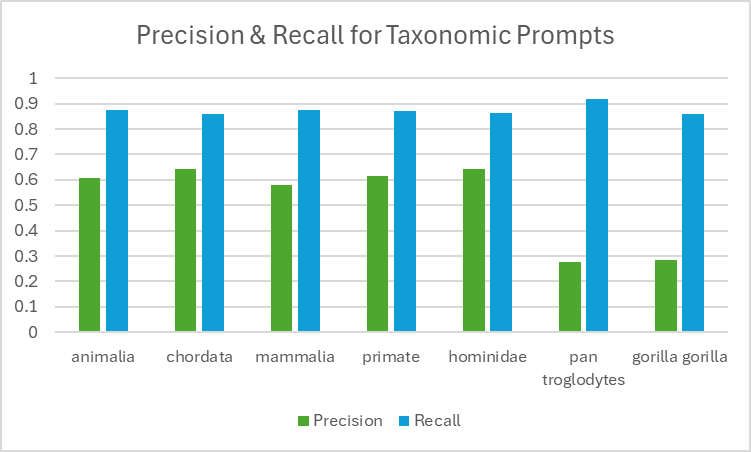
\includegraphics[width=0.75\textwidth]{images/taxonomy.png}
    \caption[Precision and Recall for Taxonomic Prompts]{Bar chart visualising the difference in precision and recall for taxonomic prompts}
    \label{fig:prompttaxonomy}
\end{figure}

The metrics shown in Table~\ref{tab:prompttaxonomy} are fairly consistent among all higher taxonomic ranks (``animalia" through ``hominidae"). When compared with the recall seen in Table~\ref{tab:metricsinitial}, however, there is no evidence to support the claim that these general prompts improve recall. Additionally, species-level precision is almost equal to that seen in Table~\ref{tab:promptformulations}

This suggests that SAM~3 does not utilise the hierarchical relationships. Instead, it seems that the model responds to general semantic associations rather than having a structured domain knowledge.

Similar to the outcome of Section~\ref{subsec:prompt_formulations}, prompts designed in this way yield varying outputs, but do not offer a practical means to improve recall or species-level precision.

\subsection{Behaviour}

An investigation into SAM~3's response to behavioural information in prompts (e.g. ``ape sitting") was executed. Since gorillas and chimpanzees can often be identified based on their behaviours (e.g. a chimpanzee is more likely to be seen climbing a tree than a gorilla would be), it was theorised that should such prompts prove effective, an ensemble model utilising behaviours and other traits could be designed as an effective two-way species classifier.


\begin{table}[h]
    \centering
    
    \begin{tabular}{ll|cccc}
        \toprule

        \textbf{Prompt} & \textbf{Ground Truth Set} & \textbf{Precision} & \textbf{Recall} & \textbf{F1} & \textbf{mAP} \\

        \midrule

        ``ape sitting" & All (sitting, sitting on back) & 0.16 & 0.93 & 0.27 & 0.33 \\

        ``ape walking" & All (walking) & 0.29 & 0.91 & 0.42 & 0.33 \\

        \bottomrule
    \end{tabular}

    \caption[Behavioural prompts]{Performance of behavioural prompts on the 71 video subset.}
    \label{tab:promptbehaviour}
\end{table}


\begin{table}[h]
    \centering

    \begin{tabular}{l|c}
        \toprule
        \textbf{Behaviour} & \textbf{Frame Count} \\
        \midrule
        Sitting (incl. on back) & 5,594 \\
        Walking & 10,913 \\
        \bottomrule
    \end{tabular}

    \caption[Dataset Behaviour Count Splits]{Disparity in number of samples featuring apes sitting compared with walking}
    \label{tab:behaviourcounts}
\end{table}

Each prompt displayed in Table~\ref{tab:promptbehaviour} yields consistently high recall and low precision, similar to what is seen with species-specific prompts.

The results indicate that SAM~3 is segmenting the subject of the prompt (``ape"), but is not distinguishing them by their actions in each video. The consistent recall but the differing precision likely does not indicate that the model is better at correctly detecting apes which are walking, but suggests the model is raising nearly all the same candidates for each prompt, it's just that PanAf71 contains a higher number of frames in which apes are walking than they are sitting. In Tables~\ref{tab:promptbehaviour}~and~\ref{tab:behaviourcounts}, we see that the ratio between precisions comes to $\approx 1.82$ and the ratio between behaviours comes to $\approx 1.95$, further supporting the claim.



\section{Species Classification}

It is clear that SAM~3 does not effectively distinguish the two ape species in the dataset. We have also shown that prompt design is not an effective method in alleviating this issue. Thus, an alternative approach must be taken in order to improve species-level classification.

This section discusses two classification models: a simple CNN built from scratch and a fine-tuned ResNet model. Each model was trained using the same data.

\subsection{Dataset}

\subsubsection{Image Preparation}

Due to SAM~3's ability to detect the majority of apes in each video, it was possible to utilise its outputs to train each model. The training setup is as follows:
\begin{enumerate}
    \item Prepare the PanAf500 videos for processing with SAM~3.
    \item Generate masklets with SAM~3's highest recall configuration (shown in Table~\ref{tab:metricsinitial}): default weights, and prompt ``ape".
    \item Verify outputs against ground truth annotations, keeping correct predictions.
    \item Crop each frame down to the corresponding bounding boxes, zeroing out the background using the predicted masks.
    \item Save each cropped region as an image, assigning an appropriate label (\texttt{chimpanzee} or \texttt{gorilla}). We will refer to these images as crops.
    \item Split into training, testing, and validation data. The validation and testing splits were made up of PanAf71 videos to avoid data leakage.
\end{enumerate}
Below are the details of each split once the crops were generated.

\begin{table}[h]
    \centering

    \begin{tabular}{l|cccc}
        \toprule
        \textbf{Split} & \textbf{Chimp Samples} & \textbf{Gorilla Samples} & \textbf{Total} & \textbf{Percentage} \\
        \midrule
        Train & 112,636 & 56,764 & 169,400 & 83\% \\
        Test & 19,349 & 9,242 & 28,591 & 14\% \\
        Validation & 3,244 & 2,446 & 5,690 & 3\% \\
        \bottomrule
    \end{tabular}

    \caption[Train, Test and Validation Split Details]{Train, Test and Validation Split Details}
    \label{tab:trainsplit}
\end{table}
% Total samples 203681

\subsubsection{Data Augmentation}

For each classification model, the following transforms were applied to the training split before training the model:
\begin{itemize}
    \item All images were resized to a resolution of $224 \times 224$ pixels.
    \item Images were horizontally flipped with a probability of $0.5$
    \item All images were rotated by a randomly selected angle between $-20^\circ$ and $20^\circ$. The small angle range ensures objects are not rotated to appear at some orientation by which they would not likely appear in any raw camera trap imagery.
\end{itemize}
Augmenting the data in such a way aims to improve the model's generalisation, consequently increasing their accuracy on unseen data.



\subsection{Training Process}

Both models were trained using the same process for the sake of comparison.

\subsubsection{Setup}

A cross entropy loss function was employed due to its effectiveness in binary classifiers \cite{crossentropy}. We adopt Adam optimisation \cite{kingma2017adammethodstochasticoptimization} with a learning rate of $1e-3$ and weight decay of $1e-5$, balancing how quickly the model learns and loss penalty size to prevent overfitting.

Additionally, we define an early stopping condition to further prevent overfitting: take the model achieving the lowest validation loss after every epoch, terminating training if there has been no improvement for a set patience level (10 epochs).

Finally, we adopt a `frame skip' parameter: this controls how many frames are skipped when preparing the dataset, aiming to reduce the data overfitting as a result of a large number of visually similar frames. For each model, the frame skip interval was set to 5.

\subsubsection{Loop}

The training loop can be described as follows:
\begin{enumerate}
    \item Prepare crops and labels
    \item Complete a forward pass through the network
    \item Compute the loss and backpropagate, updating parameters using gradient descent
    \item Measure performance on the train and validation splits using loss and classification accuracy. Accuracy was computed by taking the ratio of correct versus total predictions.
    \item Repeat until a fixed number of epochs (200) has been completed, or when the early stopping condition is met.
\end{enumerate}



\subsection{ApeNet (CNN trained solely with ape data)}

\subsubsection{Model Architecture}

Made up of four convolutional blocks followed by two full-connected layers, ApeNet is a simple CNN designed to tackle the problem at hand. Each convolutional block contains:
\begin{itemize}
    \item A convolutional layer, with a kernel of size $3 \times 3$ and padding of $1$ applied to each side.
    \item Batch normalisation (Appendix~\ref{appx:dl_functions})
    \item ReLU application (Appendix~\ref{appx:dl_functions})
    \item Max pooling with a kernel of size $2 \times 2$
\end{itemize}
After the convolutional blocks, the data is flattened and passed through the final two layers, with a dropout probability of 0.5 between each layer. Formally, the model computes:
\begin{equation}
    \label{eq:apenet}
    \textbf{x}_l = F_l(\textbf{x}_{l-1})
\end{equation}
where $\textbf{x}_{l-1}$ and $\textbf{x}_l$ are the input and output of the $l$-th layer respectively, and $F_l$ is a composite function consisting of the features described above.

\subsubsection{Performance}

\begin{table}[h]
    \centering

    \begin{tabular}{l|c}
        Loss & 26.95 \\
        \midrule
        Accuracy & 67\% \\
    \end{tabular}

    \caption[ApeNet Performance]{Performance achieved by ApeNet on the crop dataset test split.}
    \label{tab:apenetperformance}
\end{table}

\begin{figure}[h]
    \centering
    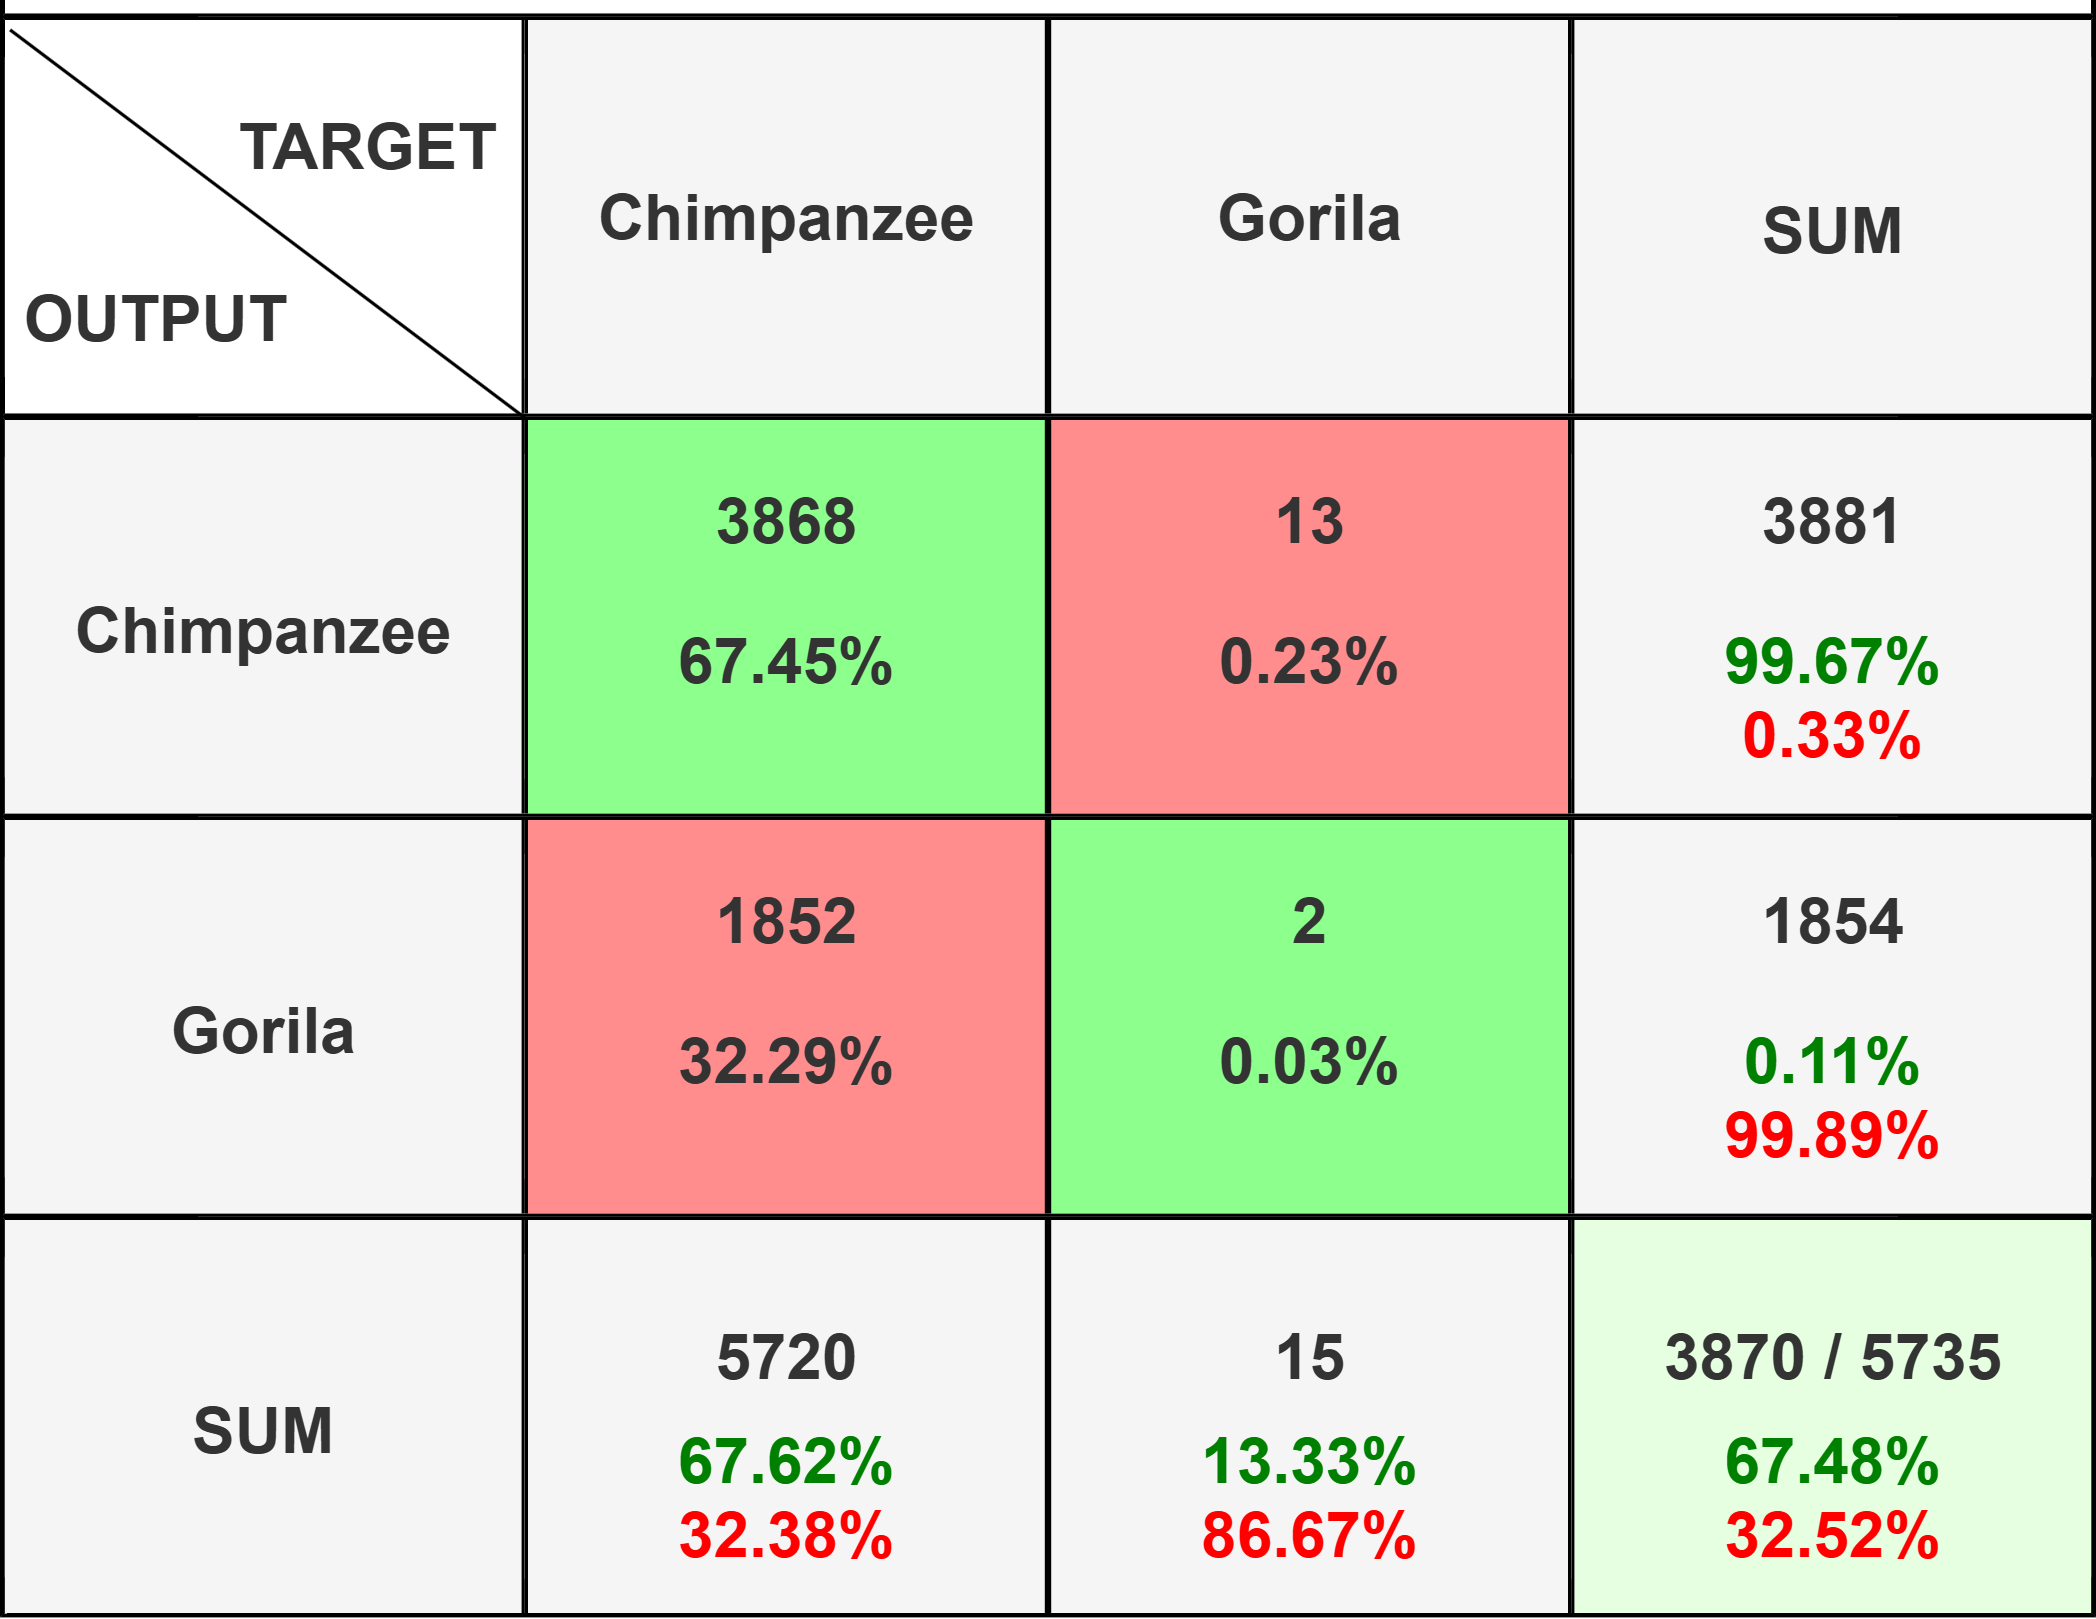
\includegraphics[width=0.6\textwidth]{images/apenet_cmatrix.png}
    \caption[ApeNet Confusion Matrix]{Confusion matrix showing ApeNet model outputs on the test split. Failures in red and successes in green.}
    \label{fig:apenetcmatrix}
\end{figure}

In Table~\ref{tab:apenetperformance}, we observe a loss of 26.95 and an accuracy score of 67\%. At first glance, the accuracy suggests that the model achieves a decent performance on the test dataset. To disprove this claim, we first acknowledge that the percentage accuracy is roughly equivalent to the percentage of samples associated with the label chimpanzee in the test split. Second, Figure~\ref{fig:apenetcmatrix} demonstrates that out of 5,375 total predictions, only 15 of those were \texttt{gorilla}, 13 of which were incorrect.




\subsection{ResNet-18 for Apes}

\subsubsection{Model Architecture}

Inspired by VGG nets \cite{simonyan2015deepconvolutionalnetworkslargescale}, ResNet is built on top of a plain network, being an initial convolutional layer and a further four residual building blocks \cite{he2015deepresiduallearningimage}. What turns this plain network into its residual counterpart, is the insertion of shortcut connections which aims to mitigate the degradation problem seen in deeper networks. The formal definition of a building block is:
\begin{equation}
    \label{eq:resnet}
    \textbf{x}_b = \mathcal{F}_b(\textbf{x}_{b-1}, \{W_i\}) + \textbf{x}_{b-1}
\end{equation}
where $\textbf{x}_{b-1}$ and $\textbf{x}_b$ are the input and output of the $b$-th block respectively, $\mathcal{F}_b$ denotes the residual mapping, and $\{W_i\}$ is the set of learnable parameters associated with $\mathcal{F}_b$. The function $\mathcal{F}_b$ represents the sequence of convolutional layers and non-linear functions such as ReLU.

This contrasts ApeNet (Equation~\ref{eq:apenet}); where ApeNet is a sequence of convolutional layers, ResNet can be thought of a sequence of blocks consisting of its own layers and shortcut connections.


\subsubsection{Fine-Tuning with Ape Data}

To adapt the model to this two-way classification problem, we replace the final fully-connected layer, reducing the number of output labels from 1000 to 2. During training, all layers of the network are updated, allowing low-level and high-level features to adapt to the domain, effective with our small number of target labels and large training dataset.


\subsubsection{Performance}

\begin{figure}[h]
    \centering
    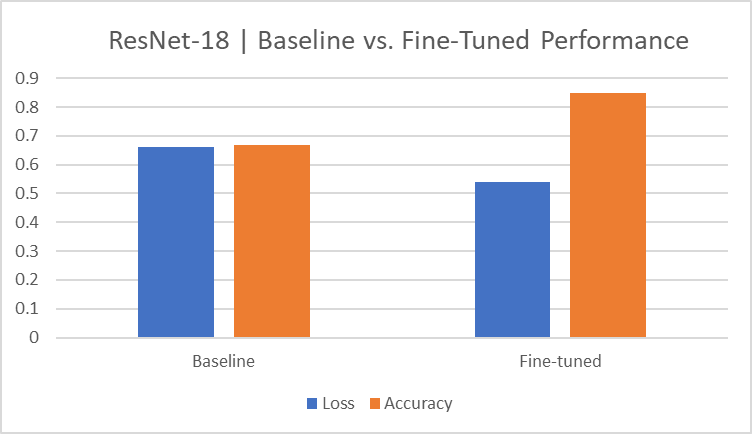
\includegraphics[width=0.75\textwidth]{images/resnet_performance.png}
    \caption[ResNet-18 Performance]{Default ResNet-18 performance, and fine-tuned performance on the crop dataset test split.}
    \label{fig:resnetperformance}
\end{figure}

Table~\ref{fig:resnetperformance} shows a performance comparison between the default ResNet-18 model initialisation, and the performance of ResNet after fine-tuning with ape data. For the baseline performance, we see a loss of 0.66 and an accuracy of 67\%. To contrast, the fine-tuned model achieved a loss of 0.54 and an accuracy of 85\%.

It is important to note that the baseline accuracy is roughly equivalent to the percentage of crops associated with the chimpanzee label. This could indicate that the model is biased towards choosing the majority class in the dataset. Thus, it is unlikely that the model is effective at differentiating between the two classes, rendering the accuracy misleading.

The additional increase of roughly 18\% in accuracy demonstrates the effectiveness of improving pre-existing models. Though the baseline is trained on a diverse dataset with many class labels, it is not optimised to effectively predict chimpanzee versus gorilla based on their visual features. Fine-tuning alleviates this issue, allowing us to purpose build the model to our use case.

\begin{figure}[h]
    \centering
    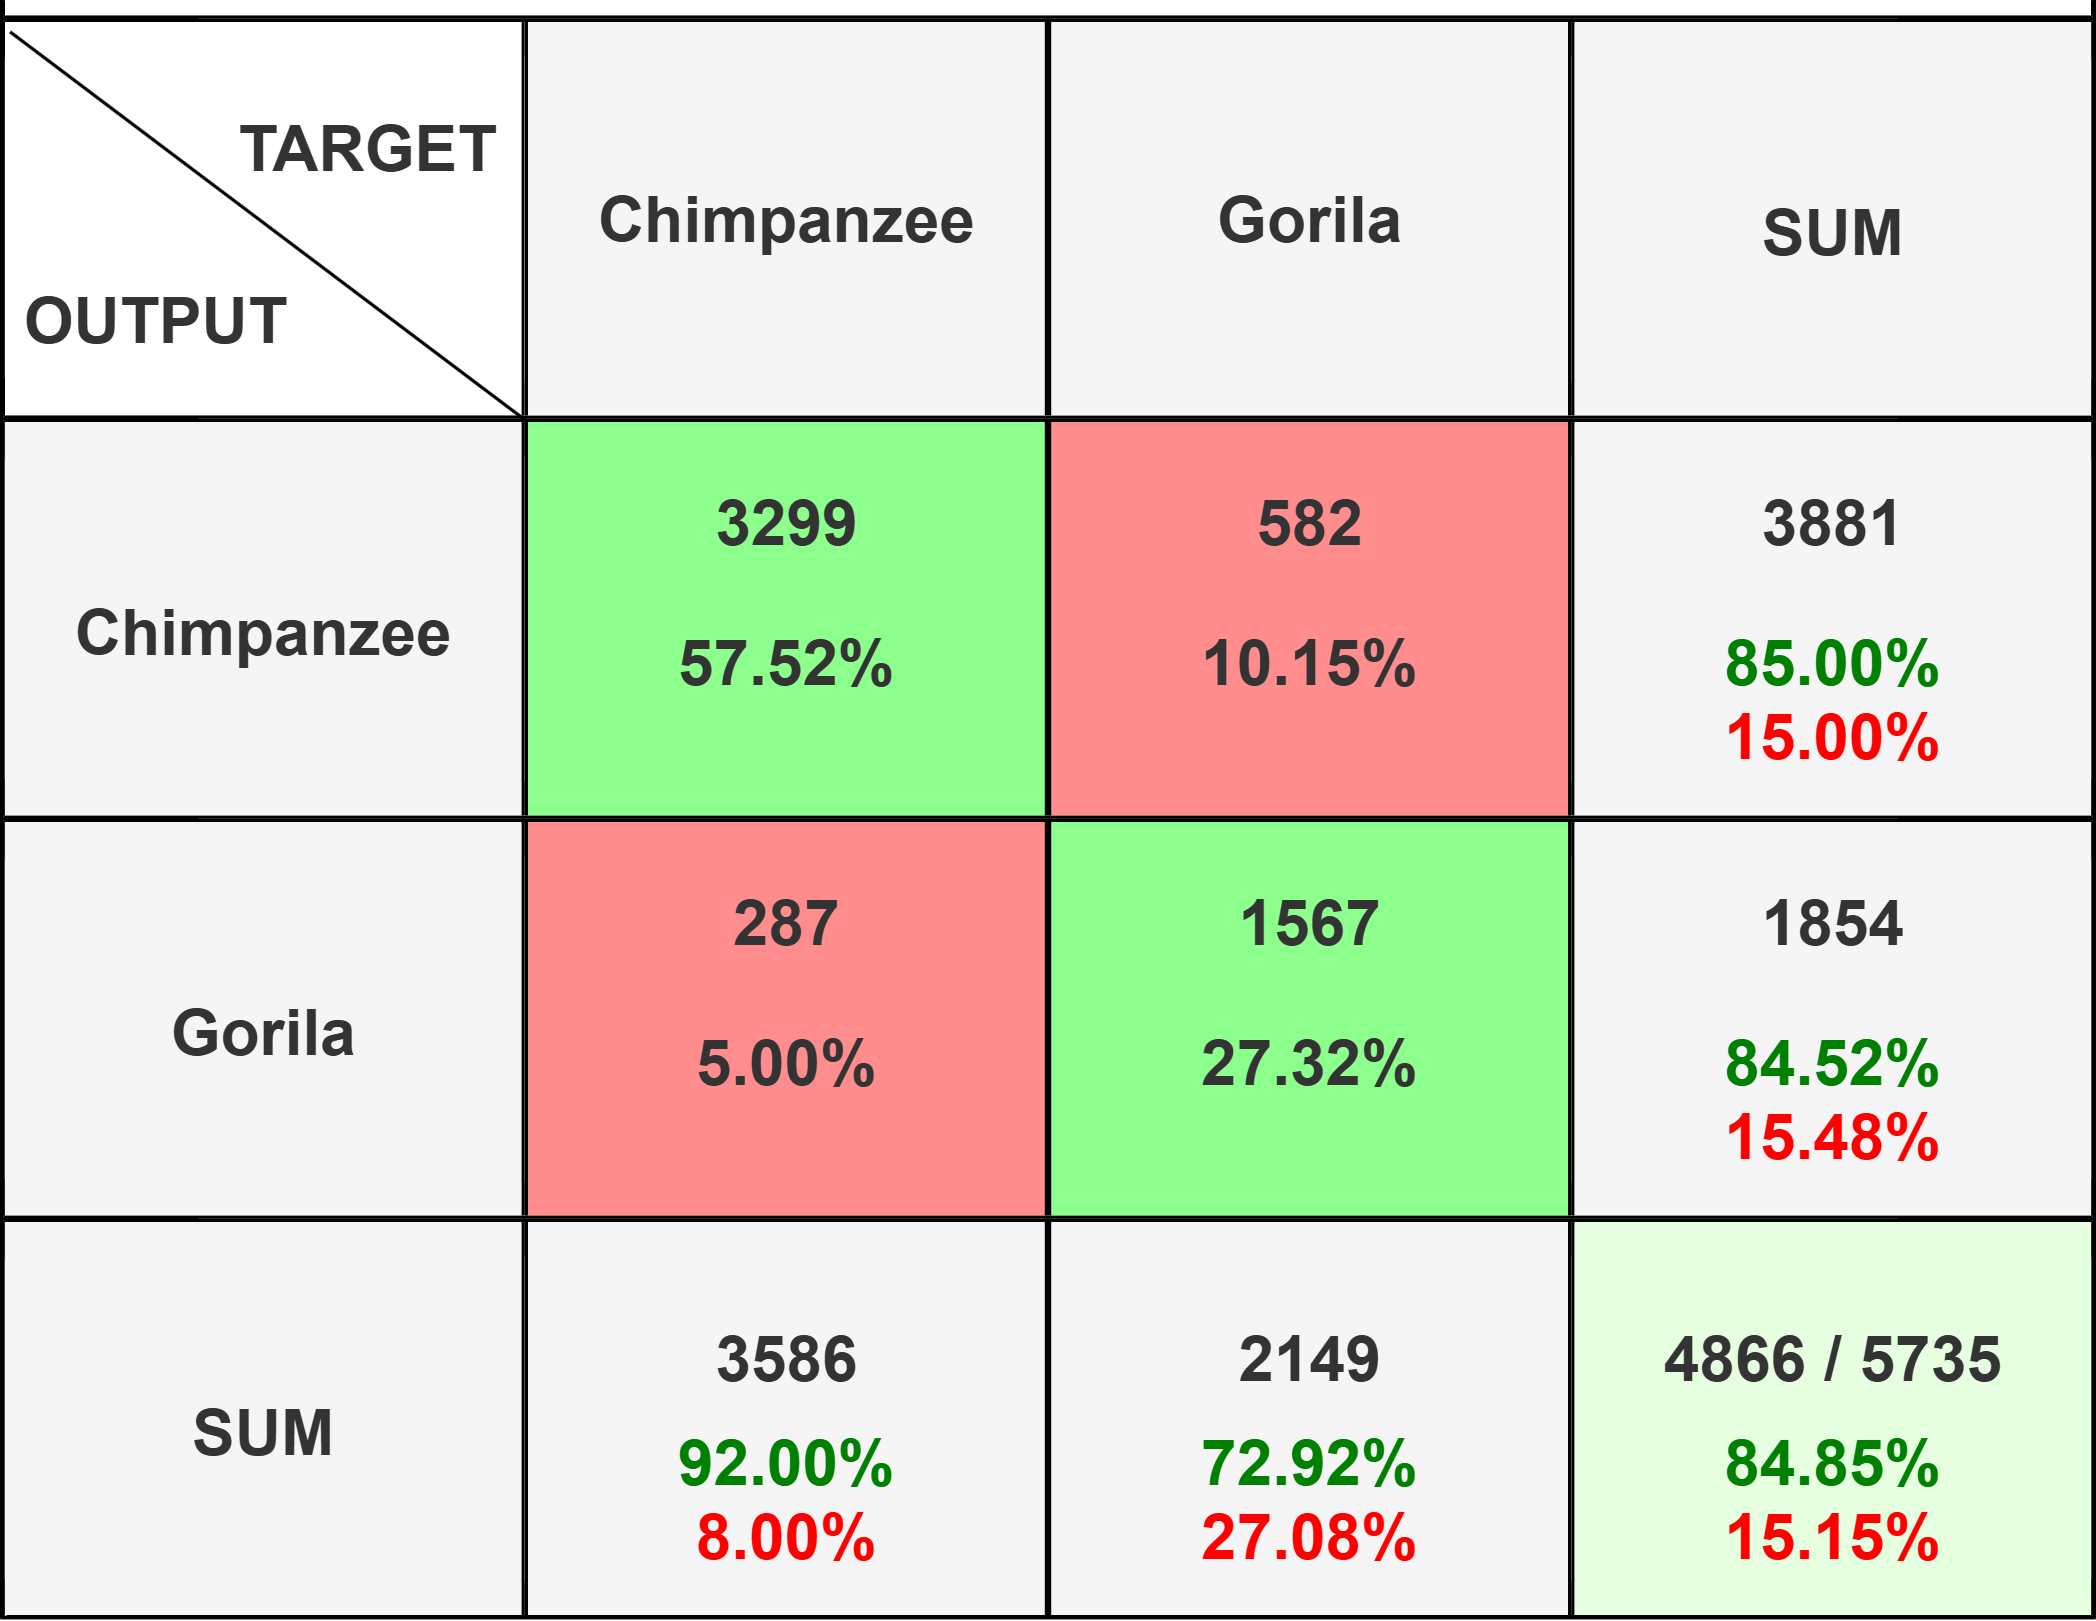
\includegraphics[width=0.6\textwidth]{images/resnet_cmatrix.png}
    \caption[Fine-Tuned ResNet-18 Confusion Matrix]{Confusion matrix showing the fine-tuned ResNet-18 model outputs on the test split. Failures in red and successes in green.}
    \label{fig:resnetcmatrix}
\end{figure}

In Figure~\ref{fig:resnetcmatrix} we see a clear difference in the number of predictions for each class when compared with Figure~\ref{fig:apenetcmatrix}. The model output \texttt{chimpanzee} 3,586 times and \texttt{gorilla} 2,149 times. This indicates that, unlike ApeNet, the model is not just outputting the majority class for almost every crop, but has learned features of each target class, and is leveraging this information when making a decision. The vast improvement can likely be attributed to the model's architecture, with more blocks / layers allowing the model to effectively learn the low and high level features.


% -----------------------------------------------------------------------------

\chapter{Critical Evaluation}
\label{chap:evaluation}


% -----------------------------------------------------------------------------

\chapter{Conclusion}
\label{chap:conclusion}



% =============================================================================

% Finally, after the main matter, the back matter is specified.  This is
% typically populated with just the bibliography.  LaTeX deals with these
% in one of two ways, namely
%
% - inline, which roughly means the author specifies entries using the 
%   \bibitem macro and typesets them manually, or
% - using BiBTeX, which means entries are contained in a separate file
%   (which is essentially a databased) then inported; this is the 
%   approach used below, with the databased being dissertation.bib.
%
% Either way, the each entry has a key (or identifier) which can be used
% in the main matter to cite it, e.g., \cite{X}, \cite[Chapter 2}{Y}.
%
% We would recommend using BiBTeX, since it guarantees a consistent referencing style 
% and since many sites (such as dblp) provide references in BiBTeX format. 
% However, note that by default, BiBTeX will ignore capital letters in article titles 
% to ensure consistency of style. This can lead to e.g. "NP-completeness" becoming
% "np-completeness". To avoid this, make sure any capital letters you want to preserve
% are enclosed in braces in the .bib, e.g. "{NP}-completeness".

\backmatter

\bibliography{dissertation}

% -----------------------------------------------------------------------------

% The dissertation concludes with a set of (optional) appendicies; these are 
% the same as chapters in a sense, but once signaled as being appendicies via
% the associated macro, LaTeX manages them appropriatly.

\appendix

\chapter{AI Prompts/Tools}
\label{appx:ai}

\section{ChatGPT}

\begin{itemize}
    \item Generated a Python script which would take a JSON file with bounding box data, and draw the bounding boxes over a copy of the corresponding video.
    \item Generated a Python script which, given a list of the PanAf500 videos used in the training of SA-FARI, copies over the videos not mentioned in the list to a new folder.
\end{itemize}



\chapter{Evaluation Metrics}
\label{appx:metrics}

This section defines the evaluation metrics used in Chapter~\ref{chap:execution}, including detection (Precision, Recall, F1, mAP) and tracking (MOTA, IDF1) performance.

\section{Detection}

\begin{table}[h]
    \centering
    
    \begin{tabular}{lcc}
        \toprule
         & \textbf{Predicted Positive} & \textbf{Predicted Negative} \\
        \midrule
        \textbf{Actual Positive} & True Positive (TP) & False Negative (FN) \\
        \textbf{Actual Negative} & False Positive (FP) & True Negative (TN) \\
        \bottomrule
    \end{tabular}
    
    \caption[Model outcomes used to evaluate detection accuracy]{Confusion matrix illustrating the outcomes used to evaluate detection accuracy.}
\end{table}

\paragraph{Precision}

Precision measures the proportion of correct predicted detections.
\begin{equation}
    \text{Precision} = \frac{TP}{TP + FP}
\end{equation}
where $TP$ denotes the number of true positives, and $FP$ denotes the number of false positives. High precision indicates that the model produces few incorrect detections.


\paragraph{Recall}

Recall measures the proportion of ground truth objects that are correctly detected.
\begin{equation}
    \text{Recall} = \frac{TP}{TP + FN}
\end{equation}
where $FN$ denotes the number of false negatives. High recall indicates that few ground truth objects go undetected.


\paragraph{F1 score}

The F1 score is the harmonic mean between precision and recall.
\begin{equation}
    F1 =
    \frac{2 \cdot \text{Precision} \cdot \text{Recall}}
    {\text{Precision} + \text{Recall}}
\end{equation}
It provides a balanced score when both precision and recall are important.


\paragraph{AP}

Average Precision measures detection accuracy across different confidence thresholds, computed as the area under the precision-recall curve.



\section{Tracking}

\paragraph{MOTA}

MOTA evaluates overall tracking accuracy by accounting for false positives, false negatives and identity switches.
\begin{equation}
    \text{MOTA} =
    1 - \frac{FN + FP + IDSW}
    {GT}
\end{equation}
where $FN$ denotes false negatives, $FP$ denotes false positives, $IDSW$ denotes the number of identity switches, and $GT$ denotes the number of ground truth objects. Higher values indicate better tracking performance.


\paragraph{IDF1}

IDF1 measures the accuracy of identity preservation during tracking.
\begin{equation}
    IDF1 = 
    \frac{2 \cdot IDTP}
    {2 \cdot IDTP + IDFP + IDFN}
\end{equation}
where $IDTP$, $IDFP$ and $IDFN$ represent identity true positives, false positives and false negatives respectively. Higher values indicate more consistent identity tracking.


\chapter{Deep Learning}
\label{appx:deeplearning}

This section provides further information on deep learning concepts.

\section{Internal Functions and Methods}
\label{appx:dl_functions}

\paragraph{ReLU}

ReLU is an activation function used for faster training and to reduce the vanishing gradient problem.
\begin{equation}
    \text{ReLU}(x) = 
    \begin{cases}
        0 & x \leq 0 \\
        x & x > 0
    \end{cases}
\end{equation}


\paragraph{Batch Normalisation}

Batch normalisation is a technique used to dramatically accelerate training of deep networks \cite{ioffe2015batchnormalizationacceleratingdeep}.
\begin{equation}
    y = \frac{x - \mathbb{E}[x]}{\sqrt{\text{Var}[x]+\epsilon}} * \gamma + \beta
\end{equation}
where $x$ is the input, $\mathbb{E}[x]$ and $\text{Var}[x]$ are the mean and variance computed per channel, $\epsilon$ is a small constant, and $\gamma$ and $\beta$ are learnable parameters.


% =============================================================================

\end{document}

% \begin{table}[h]
%     \centering

%     \begin{tabular}{ll|cccc|cc}
%         \toprule
        
%         \textbf{Prompt} & \textbf{Checkpoint} & \textbf{Precision} & \textbf{Recall} & \textbf{F1} & \textbf{mAP} & \textbf{MOTA} & \textbf{IDF1} \\
        
%         \midrule
        
%         \multirow{3}{*}{ape}
%             & SAM 3 & 0.7273 & 0.7373 & 0.7323 & 0.5977 & 0.4576 & 0.2691 \\
%             & SA-FARI & 0.7924 & 0.2678 & 0.4003 & 0.2270 & 0.1976 & 0.2004 \\
%             & SA-FARI (negs) & 0.8772 & 0.1510 &  0.2577 & 0.1318 & 0.1299 & 0.1256 \\

%         \midrule
        
%         \multirow{3}{*}{chimpanzee}
%             & SAM 3 & 0.4514 & 0.8139 & 0.5808 & 0.4266 & -0.1776 & 0.2871 \\
%             & SA-FARI & 0.7037 & 0.3602 & 0.4765 & 0.2624 & 0.2085 & 0.3263 \\
%             & SA-FARI (negs) & 0.0000 & 0.0000 & 0.0000 & 0.0000 & 0.0000 & 0.0000 \\

%         \midrule

%         \multirow{3}{*}{gorilla}
%             & SAM 3 & 0.4602 & 0.6573 & 0.5414 & 0.4680 & -0.1155 & 0.2556 \\
%             & SA-FARI & 0.3948 & 0.3997 & 0.3972 & 0.1740 & -0.2132 & 0.2796 \\
%             & SA-FARI (negs) & 0.4282 & 0.3251 & 0.3696 & 0.1903 & -0.1095 & 0.2408 \\
        
%         \bottomrule
%     \end{tabular}

%     \label{tab:findings}
%     \caption[Performance metrics for SAM 3]{Metrics quantifying SAM 3 performance on the same batch of videos for different text prompts and model checkpoints. `SAM 3' denotes the default pretrained weights. `SA-FARI' refers to weights fine-tuned using positive samples only, where `SA-FARI (negs)' indicates fine-tuning with both positives and negatives.}
% \end{table}